\documentclass[%
 reprint, amsmath,amssymb, aps, prb, ]{revtex4-2}
% 基本パッケージ
\usepackage{graphicx}
\usepackage{bm}
% 量子力学記法
\usepackage{physics}
% ハイパーリンク
\usepackage[colorlinks=true,
            linkcolor=blue, filecolor=blue, urlcolor=blue, citecolor=blue]{hyperref}
% キャプション設定
\usepackage{caption}
\captionsetup[figure]{
    justification=raggedright, labelfont={bf}, name={Fig.}, labelsep=period }
\captionsetup[table]{
    labelfont={bf}, name={Table}, labelsep=period }
% 数式番号をセクションごとに
\numberwithin{equation}{section}
% タイポグラフィ調整
\tolerance=1000
\emergencystretch=1em
\hyphenpenalty=3000
\exhyphenpenalty=3000
\flushbottom
% マイクロタイポグラフィ
\usepackage[final]{microtype}
\usepackage{ragged2e}  % for \justifying command
% \midrule、\addlinespace、\bottomruleを使う
\usepackage{booktabs}
\usepackage{enumitem}
% Theorem environment
\usepackage{amsthm}
\newtheorem{theorem}{Theorem}[section]
% Code listings with syntax highlighting
\usepackage{listings}
\usepackage{xcolor}
% 色定義 (薄いブルー系 - 学術論文向け)
\definecolor{backcolour}{rgb}{0.96,0.97,0.98}
\definecolor{deepblue}{rgb}{0,0,0.5}
\definecolor{deepgreen}{rgb}{0,0.5,0.3}
\definecolor{deepgray}{rgb}{0.4,0.4,0.4}
\definecolor{stringcolor}{rgb}{0.2,0.4,0.6}
% Pythonスタイル定義
\lstdefinestyle{pythonstyle}{
    backgroundcolor=\color{backcolour}, commentstyle=\color{deepgreen}\itshape, keywordstyle=\color{deepblue}\bfseries, numberstyle=\tiny\color{deepgray}, stringstyle=\color{stringcolor}, basicstyle=\ttfamily\footnotesize, breakatwhitespace=false, breaklines=true, captionpos=b, keepspaces=true, numbers=left, numbersep=5pt, showspaces=false, showstringspaces=false, showtabs=false, tabsize=2, language=Python, frame=single, rulecolor=\color{deepgray} }
\lstset{style=pythonstyle}
% Internal phase notation
\newcommand{\iphase}{\theta}  % internal geometric phase = ωt/2
\usepackage{tikz}
\usetikzlibrary{arrows.meta, calc, 3d, shadings, positioning, decorations.pathmorphing}

% --- Custom Macros ---
\newcommand{\omZB}{\omega_{\text{ZB}}}
\newcommand{\EphS}{E_{\text{ph}}}
\newcommand{\Egrad}{\Delta E_{\text{AB}}}
% Field strength 2-form
\newcommand{\FF}{\mathbf{F}}
% Open Wilson line
\newcommand{\WL}{\mathcal{W}}
% Hodge dual
\newcommand{\hodge}{\star}

\begin{document}

\title{Maxwell Electrodynamics as a Derived Low-Energy Limit\\
of the 0-Sphere Line-Integral Ontology}

\author{Satoshi Hanamura}
\date{April 25, 2026}

\begin{abstract}
We reformulate classical electromagnetism within the 0-Sphere model by reversing the standard ontological priority. The electromagnetic vector potential is treated not as a field defined pointwise on spacetime but as a fundamental internal 1-form $\Pi$ whose physical content is carried entirely by its integrals along open thermal geodesics. The primary observable is the open-path Wilson line $\WL[A\!\to\!A'] = \int_A^{A'}\Pi$ along the geodesic connecting the two consecutive kernel positions, with $\mathbf{r}_{A'}\neq\mathbf{r}_A$. From this single postulate the field-strength 2-form $F = d\Pi$ follows as a derived curvature, and the four Maxwell equations emerge either as mathematical identities ($dF=0$) or as stationarity conditions of the action $S=-\tfrac{1}{4\mu_0}\int F\wedge{\hodge}F$ ($d{\hodge}F=\hodge J$). The inter-kernel radiation gradient $\Egrad = E_0\cos(\omZB t)$ drives the open Wilson line $\WL(t) = W_0\sin(\omZB t)$, and the electric and magnetic fields appear, respectively, as the temporal derivative and the transverse variation of $\WL$. All gauge-invariant closed-loop observables---the Aharonov--Bohm phase and Berry-type holonomies---are shown to arise from \emph{differences} between two open path integrals that share their endpoints; no closed curve is postulated as a primary object. Maxwell electrodynamics is thereby identified as the low-energy effective description of the underlying 0-sphere internal dynamics, valid when the observation scale exceeds the kernel separation $\lambda_{\text{ZB}} = 2\pi c/\omZB$.
\end{abstract}

\maketitle

%-------------------------------------------------------------
\section{Introduction}
\label{sec:intro}
%-------------------------------------------------------------

In classical and quantum electrodynamics the field-strength tensor $F_{\mu\nu}$, or equivalently the pair $(\mathbf{E},\mathbf{B})$, is conventionally treated as the primary physical object~\cite{Jackson1998,PeskinSchroeder1995}. The vector potential $A_\mu$ is introduced as an auxiliary quantity whose gauge redundancy $A_\mu \to A_\mu + \partial_\mu\chi$ indicates that it carries more information than is directly observable. This hierarchy was challenged by the Aharonov--Bohm effect~\cite{Aharonov1959}, later confirmed experimentally by Tonomura \emph{et al.}~\cite{Tonomura1986}, which demonstrates that $A_\mu$ encodes physical information inaccessible to $F_{\mu\nu}$ alone. The standard resolution is to regard the gauge-invariant holonomy $\exp(ie\oint A_\mu\,dx^\mu/\hbar)$ as the true observable~\cite{WuYang1975}; yet this still privileges the \emph{closed-loop} integral over the connection itself.

The 0-Sphere model~\cite{hanamura01} suggests a more thoroughgoing revision of the hierarchy. Within this framework the fundamental quantity is neither $F_{\mu\nu}$ nor the holonomy, but the \emph{open-path line integral of an internal 1-form $\Pi$} along an actual physical trajectory~\cite{hanamura31}. The present paper develops this idea into a concrete reconstruction of electromagnetism. Maxwell's equations cease to be axioms of the theory: one pair follows as a mathematical identity ($dF=0$), the other pair as a variational condition ($d{\hodge}F={\hodge}J$) on an action functional built from the derived curvature. Maxwell electrodynamics is then identified as the low-energy limit of the 0-sphere dynamics, valid at scales large compared with the kernel separation $2a \sim \lambda_{\text{ZB}} = 2\pi c/\omZB \approx 3.8\times10^{-10}$~m.

The paper is organized as follows. Section~\ref{sec:motivation} explains the line-integral perspective that motivates the reformulation. Section~\ref{sec:postulate} states the physical postulate and shows how closed-loop observables such as the Aharonov--Bohm phase arise from pairs of open path integrals. Section~\ref{sec:geometry} develops the differential-form geometry. Section~\ref{sec:dynamics} connects $\Pi$ to the internal energy dynamics of the 0-sphere. Section~\ref{sec:maxwell} treats Maxwell's equations as the continuum limit of this construction. Section~\ref{sec:berry} clarifies the separation between the electromagnetic sector (open paths) and the Berry-phase sector (closed paths). Section~\ref{sec:discuss} discusses the implications, and Section~\ref{sec:conclusion} concludes. Appendices~\ref{app:algebra}--\ref{app:wave} collect algebraic and calculational details.

The exposition is self-contained. Derivations are presented in more detail than is customary for a research article, so that graduate students familiar with standard electrodynamics~\cite{Jackson1998} and elementary differential geometry~\cite{Nakahara2003} should be able to follow the argument without consulting the earlier 0-Sphere papers~\cite{hanamura01,hanamura29,hanamura30,hanamura31}.

%-------------------------------------------------------------
\section{Motivation: From Path Difference to Wilson Line}
\label{sec:motivation}
%-------------------------------------------------------------

The present work continues a sequence of studies aimed at reformulating the geometric foundations of quantum and gravitational physics~\cite{hanamura01,hanamura29,hanamura30,hanamura31}. Across these studies, the conceptual emphasis has progressively shifted from local field strengths and curvature tensors toward path-integrated phase structures, taken as the physically primary observables.

In Ref.~\cite{hanamura31}, the Aharonov--Bohm effect~\cite{Aharonov1959} was used as an illustrative case in which interference phenomena reveal the physical relevance of electromagnetic potentials even in regions where the field strength vanishes. The invariant quantity responsible for the observable phase shift is not any geometric length but the line integral of the gauge connection, namely a Wilson loop,
\begin{equation}
\Delta\phi = \frac{e}{\hbar}\oint A_\mu\,dx^\mu.
\label{eq:AB_loop}
\end{equation}
This quantity is a holonomy of the connection rather than a local curvature or metric distance~\cite{WuYang1975,Nakahara2003}.

If the Aharonov--Bohm phase demonstrates that physical geometry can reside in connection data rather than in field strength, it becomes natural to ask whether more fundamental geometric notions---such as distance and metric structure---may themselves be secondary to path-integrated phase transport. This structural question has driven the research program initiated in Ref.~\cite{hanamura01} and developed further in Refs.~\cite{hanamura29,hanamura30}.

The introduction of Wilson lines in the present paper is therefore not a merely technical reformulation. It clarifies what was structurally implicit in the previous works: what propagates between discrete kernel sites is not simply energy transfer, but phase-carrying transport encoded by an open Wilson line. The openness of this line is intrinsic to the radiation--recondensation cycle of the 0-sphere and is independent of whether the center-of-mass trajectory of the electron is closed, oscillatory, or translational.

From this perspective, the photon sphere should not be regarded as an auxiliary dynamical hypothesis. It is the concrete realization---at the Compton scale---of a path-integrated phase-transport mechanism. This reorientation allows the central working hypothesis of the present line of work to be stated sharply: \emph{path-integrated phase transport is physically primary, and local tensorial quantities are secondary descriptors of this transport}.

The structural role of line-integrated phase is not limited to Abelian gauge transport. The geometric phase discovered by Berry~\cite{Berry1984} shows that holonomy phenomena also arise in the spinorial sector. Section~\ref{sec:berry} will discuss how spinorial phase accumulation along thermal geodesics~\cite{hanamura24,hanamura26} extends the Wilson-line viewpoint beyond the U(1) case.

The remainder of the paper begins not with curvature tensors or metric postulates but with a physically operational quantity: the phase accumulated by the photon sphere as it traverses the inter-kernel geodesic of the 0-sphere.

%-------------------------------------------------------------
\section{Physical Postulate: the Open Wilson Line}
\label{sec:postulate}
%-------------------------------------------------------------

\subsection{The internal potential and its physical role}

The photon sphere carries energy between the two kernels of the 0-sphere along a definite path through space. Along this path it accumulates a geometric phase---an internal potential that we denote $\Pi$. Within the 0-Sphere model, $\Pi$ is the electromagnetic quantity closest to physical reality: it is what the photon sphere ``experiences'' along its worldline, in the same operational sense in which a charged particle in classical electrodynamics experiences the vector potential $A_\mu$. All other electromagnetic quantities---the electric and magnetic fields, and the Maxwell equations themselves---are derived consequences of $\Pi$ rather than independent physical inputs.

\subsection{The observable: phase accumulated along the open path}
\label{sec:obs}

The central physical assumption of this paper is stated as follows. The measurable electromagnetic quantity associated with one cycle of the 0-sphere is the phase accumulated by the photon sphere as it travels from the kernel position $\mathbf{r}_A$ (before the energy-exchange event) to the kernel position $\mathbf{r}_{A'}$ (after the energy-exchange event). This quantity is written as
\begin{equation}
\WL[A \to A'] \equiv \int_{\gamma:\,\mathbf{r}_A}^{\mathbf{r}_{A'}} \Pi,
\label{eq:WL}
\end{equation}
where $\gamma$ is the thermal geodesic connecting the two kernel positions. The endpoints are not arbitrary: $\mathbf{r}_A$ and $\mathbf{r}_{A'}$ are the physically determined kernel positions before and after the energy-exchange cycle, with definite internal energies $E_A$ and $E_{A'}$ given by Eqs.~\eqref{eq:EAEB} below.

A crucial structural point is that $\mathbf{r}_{A'} \neq \mathbf{r}_A$~\cite{hanamura47}: the electron is in motion, so the kernel never returns exactly to its point of departure. The path is therefore always \emph{open}. This openness is not a limitation but a structural feature. It distinguishes the electromagnetic sector, which describes a translating particle, from the spinorial sector, which describes an internal rotation~\cite{hanamura26,hanamura45}.

The strict inequality $\mathbf{r}_{A'}\neq\mathbf{r}_A$ separates the present construction from the usual treatment of Berry phase~\cite{Berry1984} or holonomy~\cite{WuYang1975}, both of which require a \emph{closed} loop with $\mathbf{r}_{\text{end}}=\mathbf{r}_{\text{start}}$. The openness is not a contingent feature of free-electron translation; it is an intrinsic property of the radiation--recondensation cycle itself. The two kernel sites $A$ and $B$, each carrying thermal potential energy and separated at the Compton-wavelength scale, exchange energy via a cycle in which the photon sphere traverses the inter-kernel geodesic and condenses its energy into the receiving kernel. Each such cycle advances the internal phase without closing it. Even when external dynamical constraints force the center-of-mass coordinate to oscillate---as for a trapped electron---the internal Wilson line $\WL[A\to A']$ remains an open path integral, because the kernel reference after recondensation carries a non-retracing phase history relative to the one before departure. It is therefore the internal phase structure, not the center-of-mass trajectory, that is categorically open (Fig.~\ref{fig:paths}).

\begin{figure*}[t]
\centering
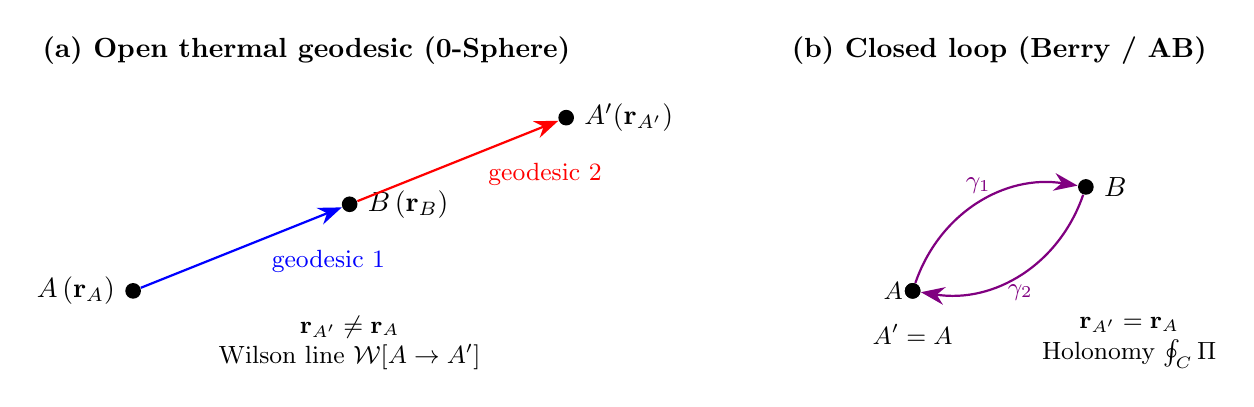
\begin{tikzpicture}[scale=1.1,
  kernel/.style={circle, fill=black, inner sep=2pt},
  arr/.style={-{Stealth[length=3mm]}, thick}
]
% --- Left panel: open path ---
\begin{scope}[xshift=-4.5cm]
\node[above] at (-1.0,2.5) {\textbf{(a) Open thermal geodesic (0-Sphere)}};
\node[kernel, label=left:{$A\,(\mathbf{r}_A)$}] (A)  at (-3,0)   {};
\node[kernel, label=right:{$B\,(\mathbf{r}_B)$}] (B) at (-0.5,1) {};
\node[kernel, label=right:{$A'(\mathbf{r}_{A'})$}] (Ap) at (2,2) {};
\draw[arr, blue, thick] (A) -- node[below right, pos=0.6, font=\small]{geodesic 1} (B);
\draw[arr, red,  thick] (B) -- node[below right, pos=0.6, font=\small]{geodesic 2} (Ap);
\node[font=\small, align=center] at (-0.5,-0.6)
  {$\mathbf{r}_{A'} \neq \mathbf{r}_A$\\Wilson line $\WL[A\to A']$};
\end{scope}
% --- Right panel: closed loop ---
\begin{scope}[xshift=2.5cm]
\node[above] at (0,2.5) {\textbf{(b) Closed loop (Berry / AB)}};
\node[kernel] (A2)  at (-1,0)   {};
\node[kernel] (Ap2) at (-1,0) {};
\node[kernel, label=right:{$B$}] (B2)  at (1,1.2) {};
\node[font=\small] at (-1,0) [left] {$A$};
\node[font=\small] at (-1,-0.5) {$A' = A$};
\draw[arr, violet, thick] (A2) to[bend left=40]
  node[above, font=\small]{$\gamma_1$} (B2);
\draw[arr, violet, thick] (B2) to[bend left=40]
  node[below, font=\small]{$\gamma_2$} (Ap2);
\node[font=\small, align=center] at (1.5,-0.6)
  {$\mathbf{r}_{A'} = \mathbf{r}_A$\\Holonomy $\oint_C \Pi$};
\end{scope}
\end{tikzpicture}
\caption{\textbf{Open vs.\ closed paths in the 0-Sphere model}}
\label{fig:paths}
\vspace{0.4em}
\begin{minipage}{0.95\textwidth}
\justifying\small
(a) The actual 0-sphere trajectory is an open thermal geodesic: after one energy-exchange cycle the photon sphere arrives at $A'$, which is spatially distinct from the starting point $A$. The open Wilson line $\WL[A\to A']$ is the primary observable. (b) Closing the path by requiring $\mathbf{r}_{A'}=\mathbf{r}_A$ produces a Berry phase or Aharonov--Bohm holonomy. In the present framework this closed object is a derived quantity obtained by comparing two open Wilson lines with the same boundary; it is not a primary postulate.
\end{minipage}
\end{figure*}

\subsection{Gauge freedom as freedom in phase reference}

The internal potential $\Pi$ is not itself directly measurable; only its integrals along physical paths are. This is reflected in the gauge freedom of the theory. Under a smooth redefinition of the phase reference $\Pi \to \Pi + d\chi$, the path integral changes only through its endpoints:
\begin{equation}
\WL[A\to A'] \;\to\; \WL[A\to A'] + \chi(\mathbf{r}_{A'}) - \chi(\mathbf{r}_A).
\label{eq:gauge_WL}
\end{equation}
Physically, this expresses the freedom to choose independent phase conventions at the two kernel positions $\mathbf{r}_A$ and $\mathbf{r}_{A'}$~\cite{hanamura17}, in parallel with the clock-synchronization picture of U(1) gauge symmetry~\cite{WuYang1975}. The only gauge-invariant quantities are \emph{differences} between two path integrals sharing the same endpoints,
\begin{equation}
\Delta\WL = \WL[\gamma_1] - \WL[\gamma_2]
= \oint_{\gamma_1\cup\overline{\gamma_2}} \Pi,
\label{eq:DeltaWL}
\end{equation}
which amounts to the circulation around the closed curve formed by the two paths. This relation is derived more carefully in the next subsection.

\subsection{Closed loops as differences of open paths: the Aharonov--Bohm connection}

In what follows we show explicitly that every gauge-invariant closed-loop observable is a \emph{derived} combination of open path integrals. This is the converse of the conventional treatment, which takes closed loops as primary. The physical picture is familiar: in the Aharonov--Bohm experiment~\cite{Aharonov1959,Tonomura1986} two electron trajectories $\gamma_1$ and $\gamma_2$ are each open paths from a source at $\mathbf{r}_A$ to a detector at $\mathbf{r}_{A'}$, and their phase difference is
\begin{equation}
H[\gamma_1, \gamma_2] \equiv \WL[\gamma_1] - \WL[\gamma_2]
= \int_{\gamma_1}\Pi \;-\; \int_{\gamma_2}\Pi.
\label{eq:H_def}
\end{equation}
We show in three steps that $H[\gamma_1,\gamma_2]$ is measurable, gauge-invariant, and equal to the magnetic flux through the enclosed surface.

\textit{Step 1 (gauge invariance).} Under $\Pi \to \Pi + d\chi$, each path integral acquires the boundary term $\chi(\mathbf{r}_{A'}) - \chi(\mathbf{r}_A)$. Since both paths share the same endpoints, these boundary terms cancel in the difference,
\begin{equation}
H \to H
+ \bigl[\chi(\mathbf{r}_{A'}) - \chi(\mathbf{r}_A)\bigr]
- \bigl[\chi(\mathbf{r}_{A'}) - \chi(\mathbf{r}_A)\bigr]
= H.
\label{eq:H_gauge}
\end{equation}
The phase difference is therefore insensitive to any choice of phase convention.

\textit{Step 2 (closed loop).} Reversing the orientation of $\gamma_2$ and appending it to $\gamma_1$ forms the closed curve $C_{12} = \gamma_1 \cup \overline{\gamma_2}$:
\begin{equation}
H[\gamma_1,\gamma_2]
= \int_{\gamma_1}\Pi + \int_{\overline{\gamma}_2}\Pi
= \oint_{C_{12}}\Pi.
\label{eq:H_loop}
\end{equation}
The closed-loop integral is not postulated here but \emph{composed} from two open paths.

\textit{Step 3 (magnetic flux).} By Stokes' theorem,
\begin{equation}
\oint_{C_{12}}\Pi = \int_{S_{12}}d\Pi = \int_{S_{12}}F = \Phi_B,
\label{eq:H_flux}
\end{equation}
where $S_{12}$ is any surface bounded by $C_{12}$ and $\Phi_B$ is the magnetic flux through it. The Aharonov--Bohm phase then follows as
\begin{equation}
\gamma_{\text{AB}} = \frac{e}{\hbar}\,H[\gamma_1,\gamma_2]
= \frac{e}{\hbar}\,\Phi_B.
\label{eq:AB_phase}
\end{equation}

Equations~\eqref{eq:H_loop}--\eqref{eq:AB_phase} show that the Aharonov--Bohm effect is simply the measurement of the phase difference between two electrons traveling along different open paths. Within this framework the closed loop and the magnetic flux are derived objects; the open path integrals are the primary physical quantities.

One may ask whether any closed loop ever forms, given that all physical geodesics satisfy $\mathbf{r}_{A'}\neq\mathbf{r}_A$. A closed loop does form, but always as a \emph{comparison} of two open paths rather than as a single closed trajectory. The Aharonov--Bohm experiment makes this concrete: the two electron arms $\gamma_1$ and $\gamma_2$ are each open, yet their combination $C_{12}$ encloses real, measurable flux. No closed geodesic is required as an independent object.

%-------------------------------------------------------------
\section{Differential-Form Geometry}
\label{sec:geometry}
%-------------------------------------------------------------

\subsection{From the 1-form to the 2-form: field strength as derived curvature}

Given the internal 1-form $\Pi$, taken to be valued in the Lie algebra of U(1) $\cong \mathbb{R}$, the \emph{field-strength 2-form} is defined as its exterior derivative~\cite{Nakahara2003,KobayashiNomizu1963},
\begin{equation}
F \equiv d\Pi.
\label{eq:F_def}
\end{equation}
This is the curvature of the connection $\Pi$ in the sense of fiber-bundle geometry~\cite{WuYang1975}. By the nilpotency of the exterior derivative, $d^2 = 0$, it follows that
\begin{equation}
dF = d(d\Pi) = 0,
\label{eq:dF_zero}
\end{equation}
which is a \emph{mathematical identity}, not a physical law. In components, $dF=0$ encodes two of Maxwell's four equations,
\begin{align}
\nabla\cdot\mathbf{B} &= 0, \label{eq:divB}\\
\nabla\times\mathbf{E} &= -\partial_t\mathbf{B}. \label{eq:Faraday_diff}
\end{align}
These relations are not postulated; they are direct consequences of the definition $F = d\Pi$. The absence of magnetic monopoles appears here as a structural property of the 1-form potential, consistent with Dirac's classic analysis~\cite{Dirac1931}.

\subsection{The action and the remaining Maxwell equations}

The remaining two Maxwell equations follow variationally from the action functional~\cite{Jackson1998,PeskinSchroeder1995}
\begin{equation}
S[\Pi] = -\frac{1}{4\mu_0}\int F\wedge{\hodge}F,
\label{eq:action}
\end{equation}
where ${\hodge}$ denotes the Hodge dual with respect to the Minkowski metric. Stationarity $\delta S/\delta\Pi = 0$ gives
\begin{equation}
d{\hodge}F = {\hodge}J,
\label{eq:dstar}
\end{equation}
where $J$ is the current 3-form. In vacuum ($J=0$) this yields
\begin{align}
\nabla\cdot\mathbf{E} &= 0, \label{eq:divE}\\
\nabla\times\mathbf{B} &= \mu_0\epsilon_0\,\partial_t\mathbf{E}. \label{eq:Ampere_diff}
\end{align}
All four Maxwell equations are therefore either mathematical identities [Eqs.~\eqref{eq:divB}--\eqref{eq:Faraday_diff}] or stationarity conditions [Eqs.~\eqref{eq:divE}--\eqref{eq:Ampere_diff}] derived from the single primary 1-form $\Pi$. None is an independent physical axiom in the present framework. Table~\ref{tab:maxwell_origin} summarizes the hierarchy.

\begin{table*}[t!]
\centering
\caption{\textbf{Ontological status of Maxwell's equations in the 0-Sphere framework}}
\label{tab:maxwell_origin}
\renewcommand{\arraystretch}{1.4}
\begin{tabular}{p{6.0cm}p{2.8cm}p{3.2cm}p{3.5cm}}
\toprule
\textbf{Maxwell equation} & \textbf{Form} & \textbf{Status} & \textbf{Origin} \\
\midrule
$\nabla\cdot\mathbf{B} = 0$
& $dF=0$ (half)
& Mathematical identity
& $d^2\Pi = 0$ \\
\addlinespace[0.3cm]
$\nabla\times\mathbf{E} = -\partial_t\mathbf{B}$
& $dF=0$ (half)
& Mathematical identity
& $d^2\Pi = 0$ \\
\addlinespace[0.3cm]
$\nabla\cdot\mathbf{E} = \rho/\epsilon_0$
& $d{\hodge}F = {\hodge}J$
& Variational condition
& $\delta S/\delta\Pi = 0$ \\
\addlinespace[0.3cm]
$\nabla\times\mathbf{B} = \mu_0\mathbf{J}+\mu_0\epsilon_0\partial_t\mathbf{E}$
& $d{\hodge}F = {\hodge}J$
& Variational condition
& $\delta S/\delta\Pi = 0$ \\
\addlinespace[0.2cm]
\bottomrule
\end{tabular}
\vspace{0.2cm}
\begin{minipage}{0.95\textwidth}
\justifying\footnotesize
Two of Maxwell's four equations are immediate consequences of $d^2=0$, requiring no physical input beyond the existence of $\Pi$. The other two follow from varying the standard electromagnetic action with respect to $\Pi$. Neither set constitutes a fundamental axiom in the 0-Sphere model; both are derived within a framework whose primary postulate is the physical picture of Sec.~\ref{sec:obs}.
\end{minipage}
\end{table*}

%-------------------------------------------------------------
\section{Internal Dynamics: Connecting $\Pi$ to the 0-Sphere Energy}
\label{sec:dynamics}
%-------------------------------------------------------------

\subsection{Energy partition and the radiation gradient}

The 0-sphere internal energy obeys~\cite{hanamura01,hanamura33}
\begin{align}
E_0 &= E_A + E_B + \EphS,\label{eq:energy}\\
E_A &= E_0\cos^4\!\!\left(\tfrac{\omZB t}{2}\right),\quad
E_B = E_0\sin^4\!\!\left(\tfrac{\omZB t}{2}\right),\label{eq:EAEB}\\
\EphS &= \tfrac{1}{2}E_0\sin^2(\omZB t).\label{eq:Eph}
\end{align}
The inter-kernel gradient
\begin{equation}
\Egrad = E_A - E_B = E_0\cos(\omZB t)
\label{eq:grad}
\end{equation}
is the driving force that propels the photon sphere along the open thermal geodesic $A\to B\to A'$. The derivation of Eq.~\eqref{eq:grad} from Eq.~\eqref{eq:EAEB} is given in Appendix~\ref{app:algebra}. The oscillation frequency $\omZB$ is the Zitterbewegung frequency, whose original introduction in the context of the Dirac equation is due to Schr\"odinger~\cite{Schrodinger1930}.

\subsection{The open Wilson line from internal dynamics}

Driven by $\Egrad \propto \cos(\omZB t)$, the photon sphere accumulates phase in quadrature (Appendix~\ref{app:response}):
\begin{equation}
\WL(t) = \int_{\mathbf{r}_A}^{\mathbf{r}_{A'}}\Pi = W_0\sin(\omZB t).
\label{eq:WL_dyn}
\end{equation}
This is the dynamical realization of the physical picture of Sec.~\ref{sec:obs}. The amplitude $W_0$ depends on the kernel separation and on the internal energy scale $E_0$.

\subsection{Electric and magnetic fields as derivatives of $\WL$}

With $\WL(t)$ as the primary quantity, the electromagnetic fields emerge as follows.

\paragraph{Electric field (temporal derivative).}
\begin{equation}
\int_{\mathbf{r}_A}^{\mathbf{r}_{A'}}\mathbf{E}\cdot d\bm{\ell}
= -\frac{d\WL}{dt} = -W_0\omZB\cos(\omZB t)
\propto -\Egrad.
\label{eq:E_from_WL}
\end{equation}
The line integral of $\mathbf{E}$ along the open geodesic equals the negative time-rate of change of the accumulated phase. The electric field is therefore the temporal derivative of the Wilson line.

\paragraph{Internal consistency check.}
The relation $-d\WL/dt \propto -\Egrad$ shows that the electromotive force along the geodesic is proportional to the very radiation gradient that drives the photon sphere along it. The field produced by the oscillation is in phase with the gradient that causes it, and $90^\circ$ out of phase with the phase accumulation itself [Eq.~\eqref{eq:WL_dyn}]. No additional physical input is needed to enforce this relation; it follows directly from differentiating $\WL(t)=W_0\sin(\omZB t)$.

\paragraph{Magnetic field (transverse variation).}
Under an infinitesimal transverse displacement $\delta\mathbf{r}_\perp$ of the geodesic enclosing an area element $\delta\Sigma$,
\begin{equation}
\frac{\partial\WL}{\partial(\delta\Sigma)}
= \int_{\delta\Sigma} F = B_\perp.
\label{eq:B_from_WL}
\end{equation}
The magnetic field is the transverse variation rate---that is, the exterior derivative in the spatial directions---of the Wilson line. It requires no specification of $\Pi(\mathbf{r})$ pointwise; it is defined through how $\WL$ changes across a family of parallel geodesics.

Equations~\eqref{eq:E_from_WL} and~\eqref{eq:B_from_WL} realize the abstract definition $F=d\Pi$ in terms of the physical open Wilson line of the 0-sphere:
\begin{equation}
\mathbf{E} = -\partial_t\Pi_{\parallel},\qquad
\mathbf{B} = \left.\frac{\partial\Pi}{\partial\mathbf{r}_\perp}\right|_{\text{transverse}},
\label{eq:EB_from_Pi}
\end{equation}
where $\Pi_{\parallel}$ denotes the component of $\Pi$ along the geodesic.

%-------------------------------------------------------------
\section{Maxwell as the Low-Energy Continuum Limit}
\label{sec:maxwell}
%-------------------------------------------------------------

Before taking the continuum limit, we clarify the geometric status of the primary observable. The Wilson line $\WL(t)$ introduced in Sec.~\ref{sec:obs} is not merely a calculational device; it reflects the $2\pi$-periodic phase structure of the model. Because physical phase is defined modulo $2\pi$, the internal configuration space has the topology of a circle $S^1$. When this phase depends smoothly on spacetime position, its periodicity naturally accommodates a U(1)-like structure~\cite{WuYang1975,Nakahara2003}. The open Wilson line may then be interpreted geometrically as the parallel transport of a circle-valued phase between two spacetime points. This interpretation highlights the compatibility of the present framework with a connection-like structure; it does not assume a pre-existing gauge field theory.

With this perspective in place, we now clarify the notion of ``discreteness'' in the 0-Sphere model before passing to the continuum limit. The model contains two kinds of structure:
\begin{enumerate}[label=(\alph*)]
\item \textit{Discrete source topology.} The two kernels constitute a zero-sphere $S^0$ (two isolated points). This discreteness is topological; it reflects the number of kernels, not any discretization of spacetime.
\item \textit{Continuous dynamics.} The radiation gradient $\Egrad = E_0\cos(\omZB t)$ is a smooth function of time. Each thermal geodesic from $\mathbf{r}_A$ to $\mathbf{r}_{A'}$ is a continuous path through unquantized space, and the Wilson line $\WL(t)=W_0\sin(\omZB t)$ is a smooth observable.
\end{enumerate}
This structure is qualitatively different from that of lattice gauge theory~\cite{Wilson1974}, where \emph{spacetime} itself is discretized and the continuum is recovered only in the zero-lattice-spacing limit. Here, spacetime is never discretized; only the source has a two-point ($S^0$) topology.

The continuum field theory emerges not from a lattice limit but from a scale separation. When the observation scale $\ell$ satisfies
\begin{equation}
\ell \gg 2a \sim \lambda_{\text{ZB}} = \frac{2\pi c}{\omZB} \approx 3.8\times10^{-10}~\text{m},
\label{eq:limit}
\end{equation}
the two-point source structure is unresolved by the observer, and the following replacements become valid.
\begin{enumerate}
\item The single Wilson line $\WL(t) = \int_{\mathbf{r}_A}^{\mathbf{r}_{A'}}\Pi$, defined on a continuous geodesic in continuous space, is extended to a smooth 1-form field $\Pi(\mathbf{r},t)$ valid across the observation region.
\item The field strength $F = d\Pi$ becomes the classical $F_{\mu\nu}$.
\item The Bianchi identity $dF=0$ and the vacuum equations $d{\hodge}F=0$ produce the full set of Maxwell equations.
\item The wave equation $\Box\Pi = 0$ in the Lorenz gauge emerges as a macroscopic consistency condition on $\Pi(\mathbf{r},t)$ in source-free regions (Appendix~\ref{app:wave}).
\end{enumerate}

\paragraph{How the interpolation works.}
Step 1 above deserves a brief clarification. The object $\WL(t)$ is a scalar defined along a specific open geodesic, whereas $\Pi(\mathbf{r},t)$ is a 1-form field defined over space. The passage from the former to the latter is not an additional dynamical postulate; it is a coarse-grained reconstruction consistent with three conditions: (i) the boundary condition $\WL(t)=W_0\sin(\omZB t)$ at the source; (ii) macroscopic causality, in the sense that no superluminal propagation is allowed; (iii) smoothness at scales $\ell \gg \lambda_{\text{ZB}}$. Under these conditions, a retarded extension
\begin{equation}
\Pi(r,t) = \frac{W_0}{r}\sin\!\left[\omZB\!\left(t-\frac{r}{c}\right)\right]
\label{eq:retarded}
\end{equation}
is selected as a causally consistent interpolation in the far-field region $r>0$. This expression satisfies $\Box\Pi=0$ away from the source and reproduces $\WL(t)$ in the near-field limit $r\to0$ within the chosen resolution scale. No claim of global uniqueness is made here; the retarded branch is simply the natural choice compatible with macroscopic causality~\cite{Jackson1998} and with the imposed boundary data.

The smooth 1-form description is thus valid precisely when $\ell\gg\lambda_{\text{ZB}}$. Below $\lambda_{\text{ZB}}$ the two kernel positions are individually resolvable, and the smooth interpolation breaks down. Maxwell electrodynamics therefore appears as the scale-separated effective theory of the 0-sphere dynamics, valid at $\ell\gg\lambda_{\text{ZB}}$. Below $\lambda_{\text{ZB}}$ the $S^0$ source topology is resolvable, and the differential-form language must be replaced by the Wilson-line description of Sec.~\ref{sec:obs}.

This geometric viewpoint clarifies why the electromagnetic sector naturally involves open Wilson lines rather than closed-loop holonomies. The distinction becomes important when comparing with Berry-type phase phenomena, to which we now turn.

%-------------------------------------------------------------
\section{Berry Phase, Holonomies, and the Spinorial Sector}
\label{sec:berry}
%-------------------------------------------------------------

The $2\pi$ periodicity underlying the electromagnetic sector admits a U(1)-like geometric interpretation. The 0-Sphere model also exhibits Berry-phase physics~\cite{Berry1984,hanamura26} in a categorically different sector.

The spinorial degree of freedom accumulates a Berry phase of $4\pi$ over a closed round-trip $A\to B\to A\to B\to A$, consisting of four geodesic segments returning to the original kernel position~\cite{hanamura29}. This is a closed-loop holonomy statement, naturally associated with SU(2) spin structure~\cite{hanamura45} and analogous to the non-Abelian holonomies familiar from Yang--Mills theory~\cite{YangMills1954}.

The electromagnetic sector, by contrast, involves open geodesics $A\to B\to A'$ with $\mathbf{r}_{A'}\neq\mathbf{r}_A$. Here the primary quantity is the open Wilson line defined relative to fixed endpoints. The two sectors are compared in Table~\ref{tab:sectors}.

\begin{table*}[t!]
\centering
\caption{\textbf{Spinorial vs.\ electromagnetic sectors of the 0-Sphere model}}
\label{tab:sectors}
\renewcommand{\arraystretch}{1.4}
\begin{tabular}{p{4.5cm}p{5.5cm}p{5.5cm}}
\toprule
\textbf{Property} & \textbf{Spinorial (Berry) sector} & \textbf{Electromagnetic (Wilson) sector} \\
\midrule
Degree of freedom
& Kernel spin
& Photon-sphere translation \\
\addlinespace[0.3cm]
Path topology
& Closed ($\mathbf{r}_{\text{end}}=\mathbf{r}_{\text{start}}$)
& Open ($\mathbf{r}_{A'}\neq\mathbf{r}_A$) \\
\addlinespace[0.3cm]
Periodicity
& $4\pi$ (spinorial, SU(2))
& $2\pi$ (bosonic, U(1)) \\
\addlinespace[0.3cm]
Primary quantity
& Holonomy $\oint\Pi$
& Wilson line $\int_A^{A'}\Pi$ \\
\addlinespace[0.3cm]
Gauge invariance
& Full (closed loop)
& Boundary-relative \\
\addlinespace[0.3cm]
Physical output
& Spin quantization, AMM
& Electric field, magnetic flux \\
\addlinespace[0.3cm]
Maxwell role
& Not applicable
& $F=d\Pi$,\quad $dF=0$ \\
\addlinespace[0.2cm]
\bottomrule
\end{tabular}
\vspace{0.2cm}
\begin{minipage}{0.95\textwidth}
\justifying\footnotesize
The spinorial and electromagnetic sectors of the 0-Sphere model employ different path topologies and yield different physical outputs. Conflating them, for instance by asking whether the electromagnetic Wilson line satisfies a $2\pi$-modular Berry condition, would be a category error. The open-path structure of the electromagnetic sector is not a weakness but a precise reflection of the photon sphere's translational motion between successive kernel encounters.
\end{minipage}
\end{table*}

%-------------------------------------------------------------
\section{Discussion}
\label{sec:discuss}
%-------------------------------------------------------------

\subsection{Topological origin of gauge invariance: from $S^0$ structure to open Wilson lines}
\label{sec:topogauge}

The central structural claim of the present framework can now be stated precisely. Gauge invariance in the electromagnetic sector originates from the $S^0$ topology of the source structure. It is not imposed as a symmetry principle at the level of a spacetime field, but emerges from the geometric constraints of a two-point source.

\paragraph{$S^0$ topology and $2\pi$ structure.}
The source consists of two discrete kernels forming a zero-sphere $S^0$. Because the photon sphere propagates continuously between these fixed endpoints, any closed round-trip trajectory necessarily returns to the same kernel position. Such closed paths define holonomies. In the spinorial sector this produces the Berry-phase structure, where only phases modulo $2\pi$, and for spinors modulo $4\pi$, are physically meaningful~\cite{Berry1984,hanamura29}. This modular structure is a direct consequence of endpoint coincidence.

\paragraph{Closed holonomy vs.\ open transport.}
The electromagnetic sector, by contrast, is defined by open thermal geodesics $A\to B\to A'$ with $\mathbf{r}_{A'}\neq\mathbf{r}_A$. The primary observable is therefore not a closed holonomy $\oint\Pi$ but the open Wilson line
\begin{equation}
\WL(t) = \int_A^{A'}\Pi.
\label{eq:WL_primary}
\end{equation}
Because the endpoints are physically fixed kernel positions, $\WL(t)$ is invariant under gauge transformations $\Pi\mapsto\Pi+d\chi$ that preserve the boundary data. Gauge invariance thus appears as a boundary-relative invariance, rather than as an abstract redundancy of description. Two 1-forms that agree on $\partial(A\to A')$ are gauge-equivalent in this sector.

\paragraph{Emergence of differential-form electrodynamics.}
When the observation scale satisfies $\ell\gg\lambda_{\text{ZB}}$, the two-point structure becomes unresolved, and the continuous interpolation $\Pi(\mathbf{r},t)$ is reconstructed from $\WL(t)$. The curvature
\begin{equation}
F = d\Pi
\label{eq:F_recall}
\end{equation}
follows as a derived object, with $dF=0$ identically. Maxwell electrodynamics then appears as the scale-separated continuum description of open Wilson-line transport between the two $S^0$ kernels.

\paragraph{Conceptual hierarchy.}
The logical chain is therefore
\begin{align}
S^0
&\;\longrightarrow\;
\text{endpoint structure}
\notag\\
&\;\longrightarrow\;
\text{open Wilson line}
\notag\\
&\;\longrightarrow\;
F=d\Pi
\notag\\
&\;\longrightarrow\;
\text{Maxwell theory}.
\label{eq:chain}
\end{align}
Closed Berry holonomies belong to a distinct sector where the endpoints coincide; open Wilson lines govern the electromagnetic sector where the endpoints differ. Conflating the two would obscure the topological origin of gauge invariance in the present model. Gauge symmetry is therefore not imposed; it is induced by the endpoint topology of the $S^0$ source.

\subsection{Priority structure: what is more fundamental than what}

The ontological hierarchy of the present framework is
\begin{align}
\underbrace{\WL(t) = \int_A^{A'}\Pi}_{\text{primary observable}}
&\;\longrightarrow\;
\underbrace{F = d\Pi}_{\text{derived curvature}}
\notag\\
&\;\longrightarrow\;
\underbrace{\mathbf{E},\mathbf{B},\,\text{Maxwell}}_{\text{low-energy limit}}.
\label{eq:hierarchy}
\end{align}
At each level, the objects are less fundamental than those to their left. Standard electromagnetism starts at the rightmost level and works leftward, recovering $A_\mu$ as a ``potential'' for $F_{\mu\nu}$ but never reaching the open Wilson line as a physical object. The 0-Sphere model starts at the leftmost level, where the physical process---the photon sphere traversing an open geodesic---directly defines the observable.

\subsection{The wave equation as integrability, not dynamics}

In the continuum limit, $\Box\Pi = 0$ in the Lorenz gauge is not a dynamical generator of the theory. It is the integrability condition that ensures the smooth 1-form field $\Pi(\mathbf{r},t)$---reconstructed from the continuous Wilson line $\WL(t)$ of the $S^0$-topology source as the observation scale is taken to $\ell\gg\lambda_{\text{ZB}}$---remains self-consistent across extended spacetime regions (Appendix~\ref{app:wave}). This is the role assigned to the source-free Maxwell equations in the conventional treatment: a consistency check rather than an independent cause.

\subsection{Experimental discriminant below $\lambda_{\text{ZB}}$}

The two frameworks agree at scales $\ell\gg\lambda_{\text{ZB}}$ and differ below. Maxwell predicts a smooth continuum field, while the 0-sphere model predicts discrete Wilson-line jumps at intervals $\Delta t \sim \pi/\omZB \approx 6.3\times10^{-19}$~s. A concrete signature is the anticorrelation between the photon-sphere population $\EphS\propto\sin^2(\omZB t)$ and the electromotive force $\mathcal{E}\propto-\cos(\omZB t)$ [Eq.~\eqref{eq:E_from_WL}] within each Zitterbewegung cycle. At sub-femtosecond time resolutions approaching $\pi/\omZB$, which remain an active target for attosecond spectroscopy~\cite{Krausz2009}, such sub-cycle structure may become accessible.

%-------------------------------------------------------------
\section{Conclusion}
\label{sec:conclusion}
%-------------------------------------------------------------

We have presented the 0-Sphere model as a line-integral foundation for electromagnetism, in which Maxwell's equations are derived consequences of a transport-theoretic postulate rather than independent axioms. The core structural results are as follows.

\begin{enumerate}
\item \textit{Primary quantity.} The open-path Wilson line $\WL[A\to A'] = \int_A^{A'}\Pi = W_0\sin(\omZB t)$, driven by the inter-kernel radiation gradient $\Egrad = E_0\cos(\omZB t)$ [Eq.~\eqref{eq:WL_dyn}]. Path openness ($\mathbf{r}_{A'}\neq\mathbf{r}_A$) is not an approximation but a geometric feature of the 0-sphere trajectory.

\item \textit{Field strength as curvature.} $F = d\Pi$ [Eq.~\eqref{eq:F_def}] is a derived 2-form. Two of Maxwell's four equations follow from $dF = d^2\Pi = 0$ as mathematical identities (Table~\ref{tab:maxwell_origin}).

\item \textit{Maxwell as variational limit.} The remaining two Maxwell equations arise as stationarity conditions of $S = -\tfrac{1}{4\mu_0}\int F\wedge{\hodge}F$ [Eq.~\eqref{eq:action}].

\item \textit{Maxwell as low-energy limit.} At scales $\ell\gg\lambda_{\text{ZB}}$ the discrete Wilson-line structure of the 0-sphere reduces to the smooth continuum of classical electrodynamics [Eq.~\eqref{eq:limit}]. The wave equation $\Box\Pi=0$ emerges as an integrability condition rather than as an independent axiom.

\item \textit{Sector separation.} Berry-phase physics (spinorial, closed loop, $4\pi$ periodicity) and electromagnetic physics (Wilson line, open path, $2\pi$ periodicity) constitute structurally distinct sectors of the 0-sphere framework and must not be conflated (Table~\ref{tab:sectors}).

\item \textit{Experimental discriminant.} Anticorrelation of $\EphS$ and $\mathcal{E}^2$ within each $\omZB$ cycle provides a potential sub-cycle signature that could distinguish the 0-sphere dynamics from classical Maxwell theory at scales $\lesssim\lambda_{\text{ZB}}$.
\end{enumerate}

Within the line-integral program initiated in Refs.~\cite{hanamura01,hanamura29,hanamura30,hanamura31}, the present paper plays the role of a concrete application: the reconstruction of Maxwell electrodynamics from open Wilson-line transport. Several structural questions---most notably whether the electromagnetic action admits a direct formulation as a functional $S[\{\WL\}]$ of open Wilson lines without passing through the intermediate 2-form $F=d\Pi$, and whether an analogous construction extends to spacetime geometry itself---are deferred to subsequent work.

\begin{acknowledgments}
This work was conducted independently by the author. During preparation, large language models were used as a pedagogical and editorial aid, primarily to verify the standard presentation of well-established results in quantum field theory and to improve the clarity and logical organization of the exposition. All physical assumptions, conceptual judgments, and the integral-based reinterpretation proposed here were formulated and assessed solely by the author.
\end{acknowledgments}

%-------------------------------------------------------------

\begin{thebibliography}{99}

% Sorted by order of first appearance in text

\bibitem{Jackson1998}
J.~D.~Jackson, \textit{Classical Electrodynamics}, 3rd ed.\ (Wiley, New York, 1998).

\bibitem{PeskinSchroeder1995}
M.~E.~Peskin and D.~V.~Schroeder, \textit{An Introduction to Quantum Field Theory} (Addison-Wesley, Reading, MA, 1995).

\bibitem{Aharonov1959}
Y.~Aharonov and D.~Bohm, ``Significance of Electromagnetic Potentials in the Quantum Theory,'' Phys.\ Rev.\ \textbf{115}, 485--491 (1959). \href{https://doi.org/10.1103/PhysRev.115.485}{doi:10.1103/PhysRev.115.485}

\bibitem{Tonomura1986}
A.~Tonomura, N.~Osakabe, T.~Matsuda, T.~Kawasaki, J.~Endo, S.~Yano, and H.~Yamada, ``Evidence for Aharonov-Bohm Effect with Magnetic Field Completely Shielded from Electron Wave,'' Phys.\ Rev.\ Lett.\ \textbf{56}, 792--795 (1986). \href{https://doi.org/10.1103/PhysRevLett.56.792}{doi:10.1103/PhysRevLett.56.792}

\bibitem{WuYang1975}
T.~T.~Wu and C.~N.~Yang, ``Concept of Nonintegrable Phase Factors and Global Formulation of Gauge Fields,'' Phys.\ Rev.\ D \textbf{12}, 3845--3857 (1975). \href{https://doi.org/10.1103/PhysRevD.12.3845}{doi:10.1103/PhysRevD.12.3845}

\bibitem{hanamura01}
S.~Hanamura, ``A Model of an Electron Including Two Perfect Black Bodies,'' Zenodo (2018). \href{https://doi.org/10.5281/zenodo.16759284}{doi:10.5281/zenodo.16759284}

\bibitem{hanamura31}
S.~Hanamura, ``Line Integrals as Fundamental Observables in Physics: A Unified Principle Behind the Aharonov--Bohm Effect, Berry Phase, and Wilson Loops,'' Zenodo (2026). \href{https://doi.org/10.5281/zenodo.18203433}{doi:10.5281/zenodo.18203433}

\bibitem{Nakahara2003}
M.~Nakahara, \textit{Geometry, Topology and Physics}, 2nd ed.\ (Institute of Physics Publishing, Bristol, 2003).

\bibitem{hanamura29}
S.~Hanamura, ``Geometric Structure of Spinorial Phase Accumulation along Thermal Geodesics,'' Zenodo (2025). \href{https://doi.org/10.5281/zenodo.18067760}{doi:10.5281/zenodo.18067760}

\bibitem{hanamura30}
S.~Hanamura, ``From Curvature to Connection: Revisiting the Geometric Origin of Conservation Laws,'' Zenodo (2026). \href{https://doi.org/10.5281/zenodo.18135855}{doi:10.5281/zenodo.18135855}

\bibitem{Berry1984}
M.~V.~Berry, ``Quantal Phase Factors Accompanying Adiabatic Changes,'' Proc.\ R.\ Soc.\ London A \textbf{392}, 45--57 (1984). \href{https://doi.org/10.1098/rspa.1984.0023}{doi:10.1098/rspa.1984.0023}

\bibitem{hanamura24}
S.~Hanamura, ``Thermal Geodesics in the 0-Sphere Model: Extending General Relativity Through Internal Thermodynamic Structure,'' Zenodo (2025). \href{https://doi.org/10.5281/zenodo.17765349}{doi:10.5281/zenodo.17765349}

\bibitem{hanamura26}
S.~Hanamura, ``Spin from Geometry: Emergence of Spin via Internal Berry Phase in the 0-Sphere Electron Model,'' Zenodo (2025). \href{https://doi.org/10.5281/zenodo.17765409}{doi:10.5281/zenodo.17765409}

\bibitem{hanamura47}
S.~Hanamura, ``Rotational Lorentz Contraction as the Geometric Origin of the Anomalous Magnetic Moment: A Structural Correspondence with the Muon Lifetime Problem,'' Zenodo (2026). \href{https://doi.org/10.5281/zenodo.19120057}{doi:10.5281/zenodo.19120057}

\bibitem{hanamura45}
S.~Hanamura, ``Open-Path Spinorial Transport in the 0-Sphere Model and the Status of Torsion: Holonomy Sufficiency,'' Zenodo (2026). \href{https://doi.org/10.5281/zenodo.18950974}{doi:10.5281/zenodo.18950974}

\bibitem{hanamura17}
S.~Hanamura, ``From Clock Synchronization to Electromagnetism: A Realist Construction of U(1) Gauge Theory,'' Zenodo (2025). \href{https://doi.org/10.5281/zenodo.17765136}{doi:10.5281/zenodo.17765136}

\bibitem{KobayashiNomizu1963}
S.~Kobayashi and K.~Nomizu, \textit{Foundations of Differential Geometry}, Vol.~I (Wiley-Interscience, New York, 1963).

\bibitem{Dirac1931}
P.~A.~M.~Dirac, ``Quantised Singularities in the Electromagnetic Field,'' Proc.\ R.\ Soc.\ London A \textbf{133}, 60--72 (1931). \href{https://doi.org/10.1098/rspa.1931.0130}{doi:10.1098/rspa.1931.0130}

\bibitem{hanamura33}
S.~Hanamura, ``Geometrical Confinement of Energy in the 0-Sphere Model: A Topological Mechanism Underlying Rest Mass and Zitterbewegung,'' Zenodo (2026). \href{https://doi.org/10.5281/zenodo.18356895}{doi:10.5281/zenodo.18356895}

\bibitem{Schrodinger1930}
E.~Schr\"odinger, ``\"Uber die kr\"aftefreie Bewegung in der relativistischen Quantenmechanik,'' Sitzungsber.\ Preuss.\ Akad.\ Wiss., Phys.-Math.\ Kl.\ \textbf{24}, 418--428 (1930).

\bibitem{Wilson1974}
K.~G.~Wilson, ``Confinement of quarks,'' Phys.\ Rev.\ D \textbf{10}, 2445--2459 (1974). \href{https://doi.org/10.1103/PhysRevD.10.2445}{doi:10.1103/PhysRevD.10.2445}

\bibitem{YangMills1954}
C.~N.~Yang and R.~L.~Mills, ``Conservation of Isotopic Spin and Isotopic Gauge Invariance,'' Phys.\ Rev.\ \textbf{96}, 191--195 (1954). \href{https://doi.org/10.1103/PhysRev.96.191}{doi:10.1103/PhysRev.96.191}

\bibitem{Krausz2009}
F.~Krausz and M.~Ivanov, ``Attosecond physics,'' Rev.\ Mod.\ Phys.\ \textbf{81}, 163--234 (2009). \href{https://doi.org/10.1103/RevModPhys.81.163}{doi:10.1103/RevModPhys.81.163}

\end{thebibliography}

%-------------------------------------------------------------
\appendix
%-------------------------------------------------------------

\section{Radiation Gradient: Algebraic Derivation}
\label{app:algebra}

This appendix provides the explicit algebraic derivation of the radiation gradient used in the main text. The purpose of this calculation is to demonstrate that the energy difference between the two kernel sites exhibits a simple harmonic structure with angular frequency $\omZB$. Let us define
\begin{equation}
\theta = \frac{\omZB t}{2}.
\end{equation}
The energies localized at the two kernel sites $A$ and $B$ scale as
\begin{equation}
E_A = E_0 \cos^4\theta, \qquad E_B = E_0 \sin^4\theta.
\end{equation}
Their difference is
\begin{align}
E_A - E_B
&= E_0\bigl(\cos^4\theta - \sin^4\theta\bigr).
\end{align}
Using the algebraic identity $a^4 - b^4 = (a^2 + b^2)(a^2 - b^2)$, one obtains
\begin{align}
\cos^4\theta - \sin^4\theta
&= \bigl(\cos^2\theta + \sin^2\theta\bigr)\bigl(\cos^2\theta - \sin^2\theta\bigr).
\end{align}
Since $\cos^2\theta + \sin^2\theta = 1$, this simplifies to
\begin{align}
\cos^4\theta - \sin^4\theta
&= \cos^2\theta - \sin^2\theta.
\end{align}
The double-angle identity $\cos(2\theta) = \cos^2\theta - \sin^2\theta$ then gives
\begin{align}
E_A - E_B
&= E_0\cos(2\theta)
= E_0\cos(\omZB t).
\end{align}
The inter-kernel energy imbalance therefore oscillates harmonically with angular frequency $\omZB$. The radiation gradient appearing in the main text is not an independent assumption but a direct algebraic consequence of the quartic trigonometric structure of the localized kernel energies. $\square$

\section{Quadrature Response of the Photon Sphere}
\label{app:response}

Regarded as a resonantly driven harmonic oscillator with natural frequency $\omZB$, the photon sphere responds in quadrature to a cosine driving force: a force $F\propto\cos(\omZB t)$ produces a steady-state displacement $x\propto\sin(\omZB t)$ with a phase lag of $\pi/2$. This is the standard result for resonance and requires no additional physical input~\cite{Jackson1998}. The amplitude $W_0$ is fixed by the internal energy scale $E_0$ and the kernel separation $2a$.

To see why the phase lag is exactly $\pi/2$ at resonance, recall the equation of motion of a driven harmonic oscillator with natural frequency $\omega_0$ and driving frequency $\omega$,
\begin{equation}
\ddot{x} + \omega_0^2\,x = A\cos(\omega t).
\label{eq:driven}
\end{equation}
For $\omega\neq\omega_0$ the particular solution is $x(t) = \tfrac{A}{\omega_0^2 - \omega^2}\cos(\omega t)$. At resonance $\omega=\omega_0$ this expression diverges, and the correct steady-state solution, obtained by introducing a damping term $2\gamma\dot{x}$, taking $\omega\to\omega_0$, and then taking $\gamma\to 0$, is
\begin{equation}
x(t) \;\xrightarrow{\omega\to\omega_0}\; \frac{A}{2\omega_0}\,t\sin(\omega_0 t).
\label{eq:resonance_grow}
\end{equation}
In the physical 0-sphere, the amplitude does not grow without bound. The energy available to the photon sphere is bounded by $\EphS \leq \tfrac{1}{2}E_0$ [Eq.~\eqref{eq:Eph}], which saturates the oscillation at $W_0$. With this saturation, the resonant response reduces to the $\sin(\omZB t)$ form of Eq.~\eqref{eq:WL_dyn}, with the expected $\pi/2$ phase lag relative to the cosine driving gradient $\Egrad = E_0\cos(\omZB t)$.

\section{Emergence of the Wave Equation in the Continuum Limit}
\label{app:wave}

In the discrete description, radiation transport is encoded in a sequence of open Wilson lines $\{\WL_n\}$ connecting successive kernel configurations. To examine the macroscopic limit of this structure, we interpolate the discrete sequence to a smooth field $\Pi(\mathbf{r},t)$, interpreted as the coarse-grained phase-transport amplitude.

In the far-field regime, where the observation point lies at a distance $r$ from the kernel axis and retardation effects dominate, the interpolated field must depend on the retarded time $t - r/c$. The simplest spherically spreading solution compatible with energy conservation is therefore
\begin{equation}
\WL(r,t) = \frac{W_0}{r}\sin\!\bigl(\omZB (t - r/c)\bigr),
\end{equation}
where $W_0$ is a normalization constant. We now show that this retarded interpolation automatically satisfies the homogeneous wave equation. Imposing the Lorenz gauge condition $\partial_\mu\Pi^\mu = 0$, one computes
\begin{equation}
\Box \Pi
= \left(\frac{1}{c^2}\frac{\partial^2}{\partial t^2} - \nabla^2 \right)\Pi.
\end{equation}
Direct substitution of the retarded form yields
\begin{equation}
\Box\Pi = 0
\end{equation}
identically. The important point is conceptual: the wave equation does not appear here as an independent dynamical postulate. Rather, it emerges as the consistency condition required for a smooth, retarded interpolation of discrete phase-transport processes~\cite{Jackson1998}. Classical wave propagation is thereby interpreted as the continuum limit of successive open Wilson-line transport.

\clearpage

\end{document}